\section*{3. ỨNG DỤNG TÍCH PHÂN ĐỂ TÍNH THỂ TÍCH VẬT THỂ}

\subsection*{a. Tính thể tích của vật thể}

\paragraph{Công thức tính thể tích của vật thể.} 
Cho một vật thể trong không gian $Oxyz$. Gọi $\mathcal{B}$ là phần vật thể giới hạn bởi hai mặt phẳng vuông góc với trục $Ox$ tại các điểm có hoành độ $x = a, x = b$. Một mặt phẳng vuông góc với trục $Ox$ tại điểm có hoành độ là $x$ cắt vật thể theo mặt cắt có diện tích là $S(x)$. Giả sử $S(x)$ là hàm số liên tục trên đoạn $[a; b]$. Khi đó thể tích $V$ của phần vật thể $\mathcal{B}$ được tính bởi công thức:
\[
V = \int_{a}^{b} S(x) \, \mathrm{d}x
\]

\paragraph{Ví dụ.} Tính thể tích của khối chóp đều có đáy là hình vuông cạnh $L$ và chiều cao là $h$.

\noindent\textbf{Giải:} 
Chọn trục $Ox$ sao cho gốc $O$ trùng với đỉnh của khối chóp và trục đi qua tâm của đáy. Khi đó, đáy của khối chóp nằm trên mặt phẳng vuông góc với $Ox$ tại $x = h$. 
Mỗi mặt phẳng vuông góc với trục $Ox$ tại điểm có hoành độ bằng $x$ ($0 \le x \le h$), cắt khối chóp theo mặt cắt là hình vuông có cạnh là $a$. 
Theo định lí Thales, ta có $\frac{x}{h} = \frac{a}{L}$, suy ra $a = \frac{L}{h}x$. 
Do đó, diện tích của mặt cắt này là $S(x) = a^2 = \frac{L^2}{h^2}x^2$. 

Vậy thể tích của khối chóp này là:
\[
V = \int_{0}^{h} S(x) \, \mathrm{d}x = \int_{0}^{h} \frac{L^2}{h^2}x^2 \, \mathrm{d}x = \left. \frac{L^2}{h^2} \frac{x^3}{3} \right|_{0}^{h} = \frac{1}{3}L^2h.
\]

\begin{center}
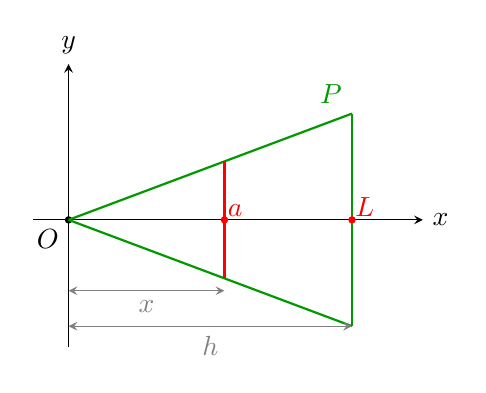
\begin{tikzpicture}[scale=0.9, >=stealth]
    % Trục tọa độ
    \draw[->] (-0.5,0) -- (5,0) node[right] {$x$};
    \draw[->] (0,-1.8) -- (0,2.2) node[above] {$y$};
    \fill (0,0) circle (1.5pt) node[below left] {$O$};
    
    \def\h{4}
    \def\px{2.2}
    
    % Tam giác cắt (màu xanh lá)
    \draw[green!60!black, thick] (0,0) -- (\h, 1.5) node[above left] {$P$};
    \draw[green!60!black, thick] (0,0) -- (\h, -1.5);
    \draw[green!60!black, thick] (\h, 1.5) -- (\h, -1.5);
    
    % Đoạn thẳng mặt cắt a tại x (màu đỏ)
    \draw[red, thick] (\px, 0.825) -- (\px, -0.825);
    % Đặt chữ a thấp xuống sát trục Ox
    \node[red, above right, inner sep=1pt] at (\px, 0) {$a$};
    \fill[red] (\px, 0) circle (1.5pt);
    
    % Điểm L trên trục Ox và đặt chữ L sát trục Ox
    \fill[red] (\h, 0) circle (1.5pt);
    \node[red, above right, inner sep=1pt] at (\h, 0) {$L$};
    
    % Các đường gióng kích thước x và h ở phía dưới
    \draw[gray, thin, <->] (0, -1.0) -- (\px, -1.0) node[midway, below] {$x$};
    \draw[gray, thin, <->] (0, -1.5) -- (\h, -1.5) node[midway, below] {$h$};
\end{tikzpicture}
\end{center}

\paragraph{Chú ý.} Bằng ứng dụng của tích phân, người ta chứng minh được thể tích của khối chóp bất kì bằng $\frac{1}{3}$ diện tích mặt đáy nhân với chiều cao của nó.

\vspace{0.5cm}

\subsection*{b. Tính thể tích khối tròn xoay}

\paragraph{Công thức tính thể tích khối tròn xoay.} 
Cho hàm số $f(x)$ liên tục, không âm trên đoạn $[a; b]$. 
Khi quay hình phẳng giới hạn bởi đồ thị hàm số $y = f(x)$, trục hoành và hai đường thẳng $x = a, x = b$ quanh trục hoành, ta được hình khối gọi là \textbf{khối tròn xoay}. 
Khi cắt khối tròn xoay đó bởi một mặt phẳng vuông góc với trục $Ox$ tại điểm $x \in [a; b]$ được một hình tròn có bán kính $f(x)$. Thể tích của khối tròn xoay này là:
\[
V = \pi \int_{a}^{b} f^2(x) \, \mathrm{d}x
\]

\paragraph{Ví dụ.} Tính thể tích khối tròn xoay sinh ra khi quay quanh trục $Ox$ hình phẳng giới hạn bởi đồ thị hàm số $y = \sqrt{x}$, trục hoành và hai đường thẳng $x = 0, x = 1$.

\noindent\textbf{Giải:} 
Thể tích khối tròn xoay cần tính là:
\[
V = \pi \int_{0}^{1} f^2(x) \, \mathrm{d}x = \pi \int_{0}^{1} (\sqrt{x})^2 \, \mathrm{d}x = \pi \int_{0}^{1} x \, \mathrm{d}x = \left. \pi \frac{x^2}{2} \right|_{0}^{1} = \frac{\pi}{2}.
\]

\begin{center}
\begin{tikzpicture}
    \begin{axis}[
        xmin=-0.5, xmax=1.5,
        ymin=-1.2, ymax=1.5,
        axis lines=middle,
        xlabel=$x$, ylabel=$y$,
        xtick={1},
        ytick={},
        samples=100,
        width=8cm, height=6cm,
    ]
        \addplot[name path=f, blue, domain=0:1.2] {sqrt(x)};
        \addplot[name path=axis, draw=none, domain=0:1.2] {0};
        \addplot[orange!60] fill between[of=f and axis, domain=0:1];
        \node[blue, font=\small] at (axis cs:0.7, 1.0) {$y = \sqrt{x}$};
        \draw[dashed, thick] (axis cs:1,0) -- (axis cs:1,1);
    \end{axis}
\end{tikzpicture}
\end{center}
